% ****** Start of file apssamp.tex ******
%
%   This file is part of the APS files in the REVTeX 4.1 distribution.
%   Version 4.1r of REVTeX, August 2010
%
%   Copyright (c) 2009, 2010 The American Physical Society.
%
%   See the REVTeX 4 README file for restrictions and more information.
%
% TeX'ing this file requires that you have AMS-LaTeX 2.0 installed
% as well as the rest of the prerequisites for REVTeX 4.1
%
% See the REVTeX 4 README file
% It also requires running BibTeX. The commands are as follows:
%
%  1)  latex apssamp.tex
%  2)  bibtex apssamp
%  3)  latex apssamp.tex
%  4)  latex apssamp.tex
%
\documentclass[%
 reprint,
%superscriptaddress,
%groupedaddress,
%unsortedaddress,
%runinaddress,
%frontmatterverbose, 
%preprint,
%showpacs,preprintnumbers,
%nofootinbib,
%nobibnotes,
%bibnotes,
 amsmath,amssymb,
 aps,
%pra,
%prb,
%rmp,
%prstab,
%prstper,
%floatfix,
]{revtex4-1}

\usepackage{graphicx}% Include figure files
\usepackage{dcolumn}% Align table columns on decimal point
\usepackage{bm}% bold math
%\usepackage{hyperref}% add hypertext capabilities
%\usepackage[mathlines]{lineno}% Enable numbering of text and display math
%\linenumbers\relax % Commence numbering lines

%\usepackage[showframe,%Uncomment any one of the following lines to test 
%%scale=0.7, marginratio={1:1, 2:3}, ignoreall,% default settings
%%text={7in,10in},centering,
%%margin=1.5in,
%%total={6.5in,8.75in}, top=1.2in, left=0.9in, includefoot,
%%height=10in,a5paper,hmargin={3cm,0.8in},
%]{geometry}
\usepackage{pstricks,pst-node}
\usepackage[utf8]{inputenc}
\usepackage{float}
\usepackage[spanish]{babel}
\usepackage{amsmath}
\usepackage{hyperref}
\usepackage{tikz}
\usepackage{tabularx}
\usepackage{graphicx}
\usepackage{adjustbox}

\begin{document}

\title{Espectros de átomos y LEDs}% Force line breaks with \\

\author{Maria Sofía Álvarez López}%
\affiliation{
 Universidad de los Andes\\
}%

\author{Sara María Varón Echeverri}
\affiliation{
Universidad de los Andes\\
}%

\date{\today}% It is always \today, today,
             %  but any date may be explicitly specified

\begin{abstract}
Los objetivos para este laboratorio fueron principalmente tres. Primero, se midieron las longitudes de onda emitidas por el hidrógeno y se comprobó con éxito el ajuste de la fórmula de Balmer. Esto se demuestra con el coeficiente de correlación presentado en la gráfica: 0.9488. Los datos encontrados se muestran precisos y exactos conforme a los valores esperados. Segundo, se determinó la constante de Rydberg con un error de $7.998\%$. La regresión lineal correspondiente presenta un valor de $0.010096 nm^{-1}$ que se aleja del valor teórico por errores aleatorios tales como el paralaje y el error asociado a los instrumentos de medida. Tercero, se midieron satisfactoriamente algunas líneas espectrales del mercurio, neón, helio y del argón. Los valores de error asociados a estos datos son todos menores al $10\%$, demostrando ser datos con una precisión aceptable y moderada teniendo en cuenta el modelo planteado. Adicionalmente, se midieron las longitudes de onda emitidas por varios LEDs: uno azul, uno verde y uno amarillo. Para todos los casos, se determinó el rango de longitudes de onda en el que se difractaba el espectro de cada uno y el punto donde había mayor intensidad lumínica. Para todos los casos, se obtuvieron errores experimentales menores al $5\%$, evidenciando una gran exactitud de los datos respecto a los valores aceptados. Es por este error que el rango encontrado realmente correspondía al color inmediatamente siguiente (para el amarillo y el verde) o anterior (para el azul) en el espectro de luz visible. A pesar de lo anterior, el experimento en su totalidad fue exitoso y evidenció gran exactitud en los resultados obtenidos. 
\end{abstract}

\pacs{Valid PACS appear here}% PACS, the Physics and Astronomy
                             % Classification Scheme.
%\keywords{Suggested keywords}%Use showkeys class option if keyword
                              %display desired
\maketitle

%\tableofcontents

\section{\label{sec:introduccion} Introducción y estado del arte}

Cada elemento en su estado gaseoso tiene en un espectro de líneas ciertas longitudes de ondas \cite{fisicauniversitaria}. Un gas calentado emite ciertas longitudes de ondas mientras que un gas frío absorbe diversas longitudes de onda, consecuentemente, se le denota respectivamente a cada set de longitudes de onda el espectro de emisión y el espectro de absorción. Gracias a esto, se lograron descubrir diversos elementos y se pudo estudiar a cabalidad los átomos de los elementos ya existentes conforme a su composición. 

\begin{figure}[H]
    \centering
    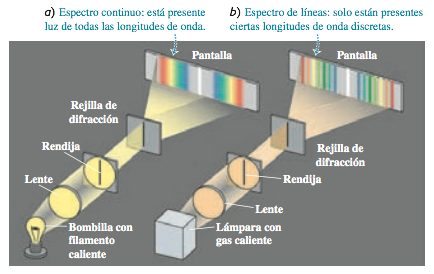
\includegraphics[scale= 0.5]{espectro_de_lineas.png}
    \caption{Espectro de líneas que se generan conforme a una lámpara de gas \cite{fisicauniversitaria}.}
    \label{fig:espectro}
\end{figure}


Diversos científicos se pusieron entonces a la tarea de estudiar el átomo del Hidrógeno, ya que éste era el elemento con mayor abundancia en el universo. Entre esos, Anders Ångström había logrado encontrar cuatro líneas visibles en el espectro atómico del hidrogeno y Johann Jakob Balmer había generalizado sus descubrimientos en un fórmula que predecía las longitudes de onda de su experimento, como se muestra en \eqref{Balmer} \cite{serway2004modern}. Cabe notar que la ecuación está escrita para longitudes de onda en centímetros, y que $C_2$ es la constante del límite de convergencia, con un valor aproximado en $3645.6 \times 10^{-8} cm$.

\begin{equation} \label{Balmer}
   \lambda = C_2 \left(\frac{n^2}{n^2-2^n}\right)
\end{equation}

Ahora, al generalizar la expresión de Balmer, se encontró que la mejor manera de describir las longitudes de onda sería con la ecuación \eqref{BalmerMejorada}, donde R es la constante de Ryderberg con un valor aproximado de $0.010973732 nm^{-1}$.

\begin{equation} \label{BalmerMejorada}
   \frac{1}{\lambda} = R \left(\frac{1}{n_f^2} - \frac{1}{n_i^2} \right)
\end{equation}

\begin{figure}[H]
    \centering
    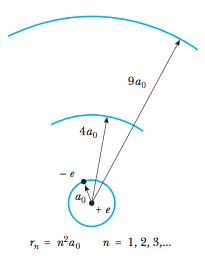
\includegraphics[scale= 0.5]{orbitas_Bohr.png}
    \caption{Los primeros tres radios de Bohr \cite{serway2004modern}.}
    \label{fig: radios de Bohr}
\end{figure}

Tras estas investigaciones, Niels Bohr publicó su trabajo ``On the Constitution of Atoms and Molecules'' en 1913. En éste trabajo se discute una posible solución al modelo del electrón que perdía de manera indefinida energía y se plantean los estados estacionarios: niveles de energía estables en los que no hay radiación \cite{Bohr}. Dado lo anterior, continuó su estudio detallado sobre el átomo de hidrógeno y llegó a diversas conclusiones. Por un lado, encontró que sólo ciertos radios del átomo de hidrógeno aceptaban aquellos estados estacionarios y los describió con la ecuación \eqref{radiosBohr}. Algunos de estos son ilustrados en la figura \ref{fig: radios de Bohr}, siendo $a_0$ el "Radio de Bohr" con un valor de $0.0529 nm$. Por otro lado, halló que la ecuación que mejor describía la emisión de las longitudes de onda para el hidrógeno \eqref{ecuacionBohr}, igual a la ecuación presentada por Balmer anteriormente \eqref{BalmerMejorada}.

\begin{equation} \label{radiosBohr}
   r_n = \frac{n^2 \hbar^2}{m_eke^2}
\end{equation}

\begin{equation} \label{ecuacionBohr}
   \frac{1}{\lambda} = \frac{ke^2}{2a_0hc} \left(\frac{1}{n_f^2} - \frac{1}{n_i^2} \right)
\end{equation}

Por otro lado, una rendija (o también llamada rejilla) de difracción es un material que cuenta con múltiples ranuras paralelas, todas del mismo tamaño (a) y separadas por la misma distancia (d). Esto cumple con la ecuación \eqref{(2)}, que toma en cuenta las frecuencias pueden ser constructivas o destructivas dependiendo del ángulo que se forma entre ellas. 

\begin{equation} \label{(2)}
    d \sin \theta = m\lambda
\end{equation}

En este experimento en particular, se analizarán los espectros de emisión de 5 elementos diferentes: Mercurio (Hg), Helio (He), Hidrógeno (H), Neón (Ne) y Argón (Ar). Los espectros asociados a cada uno se presentan a continuación: \\

\begin{figure}[H]
    \centering
    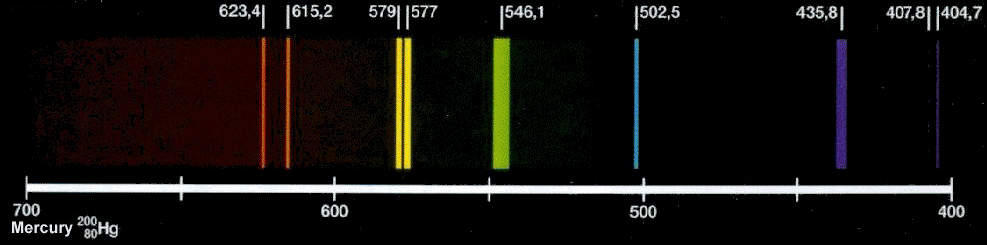
\includegraphics[scale= 0.3]{mercurio.png}
    \caption{Esta imagen muestra el espectro de emisión del Mercurio (Mg). En este, se muestran dos lineas espectrales rojas, 2 amarillas, 1 verde y 1 morada.}
    \label{fig: Hg}
\end{figure}
\begin{figure}[H]
    \centering
    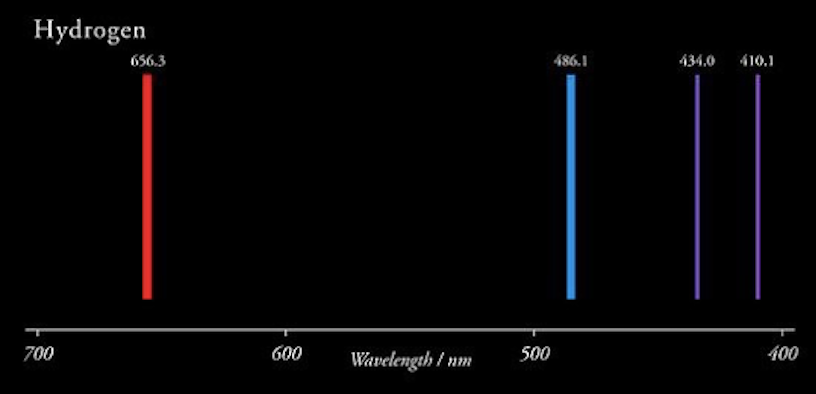
\includegraphics[scale= 0.5]{hydrogen.png}
    \caption{Esta imagen muestra el espectro de emisión del Hidrógeno (H). En este, se muestra una linea espectral roja, 1 azul y 2 moradas. }
    \label{fig: H}
\end{figure}
\begin{figure}[H]
    \centering
    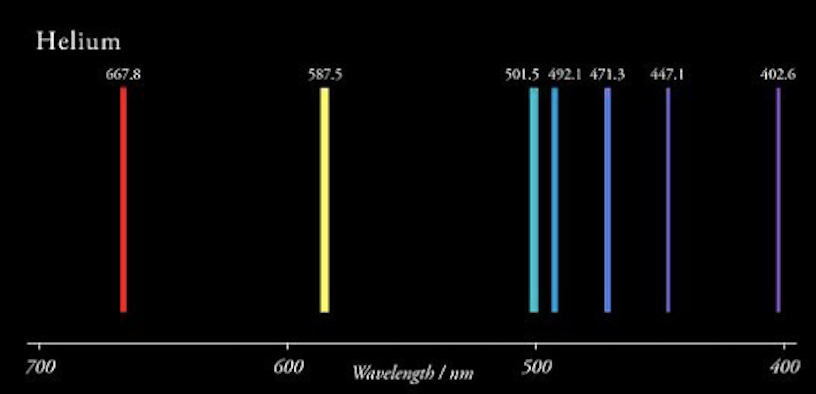
\includegraphics[scale= 0.5]{helium.png}
    \caption{Esta imagen muestra el espectro de emisión del Helio (He). En este, se muestra una linea espectral roja, una amarilla, una azul clara, dos azules oscuras y dos moradas. Es muy posible que la última línea espectral morada, con $\lambda_{Teorico} = 402.6 nm$ no pueda verse, porque está muy cerca del inicio del espectro ultravioleta.}
    \label{fig: He}
\end{figure}
\begin{figure}[H]
    \centering
    
\includegraphics[scale= 0.58]{neon.png}
    \caption{Esta imagen muestra el espectro de emisión del Neón (Ne). En este, se observa una línea espectral verde, una amarilla, una naranja y varias tonalidades de rojo. Es bastante posible que las últimas líneas del rojo no puedan observarse pues están muy cerca al espectro del infrarrojo.}
    \label{fig: Ne}
\end{figure}

\begin{figure}[H]
    \centering
    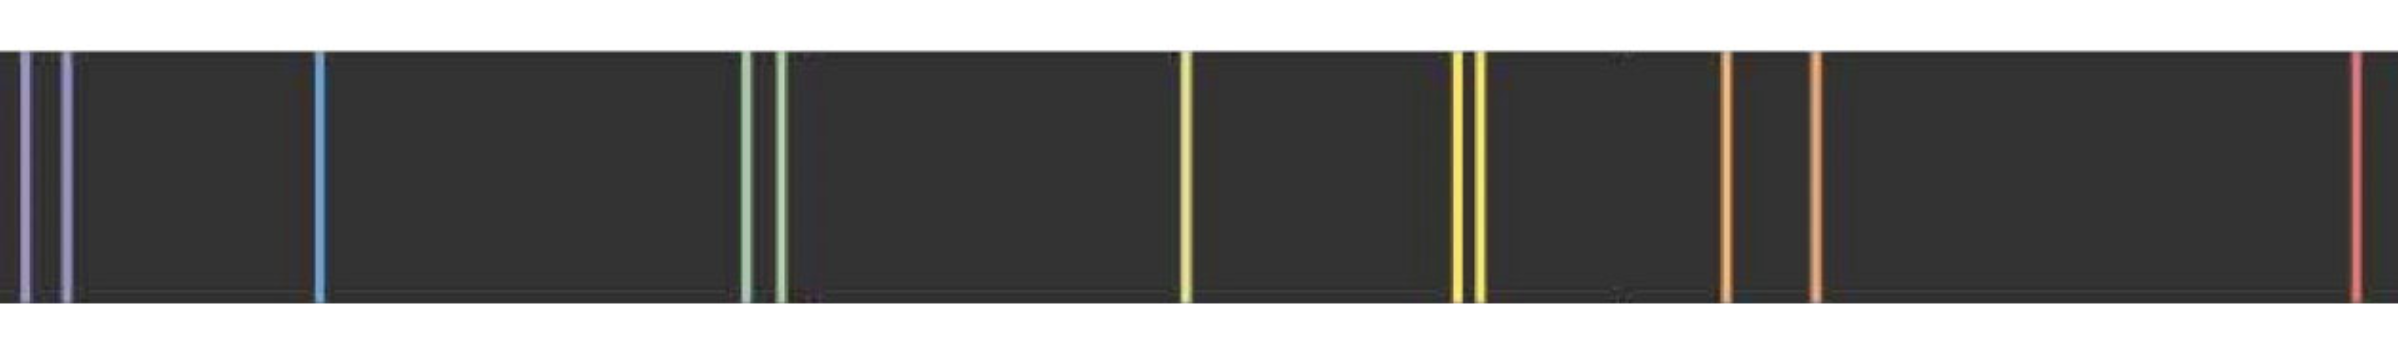
\includegraphics[scale= 0.2]{argon.png}
    \caption{Esta imagen muestra el espectro de emisión del Argón (Ar). En este, se observa una línea espectral azul, dos verdes, 3 amarillas, 1 naranja, otra naranja-rojiza y una última roja.}
    \label{fig: Ar}
\end{figure}


Finalmente, teniendo en cuenta que se utilizarán LEDs, es importante explicar su naturaleza y características importantes para el desarrollo del experimento. La palabra "LED" viene de las siglas en inglés para "light-emitting diodes". Estos son bombillos que no gastan energía en calor dado que no están hechos de un filamento sino que proveen luz mediante el desprendimiento de electrones de un material semiconductor que no genera campos electrostáticos que puedan afectar mediciones en el laboratorio \cite{Leds_semiconductores}. Una de las razones por las cuales se utilizan este tipo de bombillos y no otros es por su luminosidad y que pueden encenderse en menos de 1 $\mu s$ que responde de forma beneficiosa al tiempo de respuesta de los experimentos \cite{LEDs}. Adicionalmente, son luces monocromáticas, en otras palabras, sólo tienen una longitud de onda específica que puede ser estudiada con claridad asociada al color del bombillo. La estrechez del espectro de los LED es una característica única de éstos elementos y se presenta como una característica fundamental para el desarrollo de los experimentos \cite{LED_monocromatico}.
\\
\section{\label{sec:montaje} Montaje experimental}
Para este experimento, el primer paso realizado fue hacer el montaje experimental mostrado en la imagen \ref{fig:diagrama} mostrada a continuación. 
\begin{figure}[H]
    \centering
    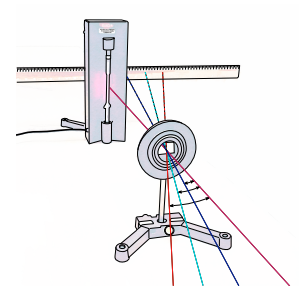
\includegraphics[scale= 0.65]{Montaje.png}
    \caption{Montaje experimental con tubos espectrales y su fuente. Como se ve en la imagen, es posible analizar los espectros de diferentes elementos (con lámparas que están hechas de ellos) utilizando una rejilla de difracción. Un proceso similar se realizó con los LEDs.}
    \label{fig:diagrama}
\end{figure}
Cabe aclarar que, para medir las posiciones de cada linea espectral, se puso una regla perpendicular a la línea visual (Esto también puede verse en la imagen \ref{fig:diagrama}). Asimismo, se midió la distancia entre la regla y la rejilla de difracción. Se notó que, entre más grande fuera esta distancia \textit{L}, era más sencillo notar las separaciones entre las líneas espectrales. Sin embargo, esto resultaba en que no se pudieran ver todas las líneas espectrales para cada elemento ni determinar, con exactitud, su posición sobre la regla. No obstante, se decidieron tomar dos sets de datos, para cada lámpara, con longitudes de $L=149,2 cm$ y $L=18,5 cm$, con el fin de escoger los datos, para cada linea espectral, cuya longitud de onda estuviese más cercana a los valores de referencia de la NIST, para cada lámpara. \\
Cabe aclarar que este proceso se realizó para 5 tubos espectrales, de Argón (Ar), Mercurio (Mg), Helio (He), Neón (Ne) e Hidrógeno (H). Cabe aclarar que, debido a la naturaleza del primero, sólo se pudieron calcular las longitudes de onda, $\lambda$, para $L=18,5 cm$; puesto que, para $L=149,2 cm$, las líneas eran bastante difusas y no podía establecerse, con exactitud, su posición sobre el instrumento de medición (la regla). Por su parte, para el último, se calcularon las longitudes de onda, $\lambda$, y se graficaron contra n, convirtiendo la fórmula de Balmer en una relación lineal adecuada cuya pendiente corresponda a la constante de Rydberg. Cabe aclarar que, para los cálculos para la longitud de onda de cada línea espectral de cada elemento, se encontró, primero, el ángulo con el que cada color se desviaba al pasar por la rejilla. Así, utilizando la ecuación \eqref{(2)}, podía encontrarse la longitud de onda asociada a cada una, utilizando m=1.\\
Finalmente, se realizó un proceso similar al de las lámparas, con 3 LEDs: uno verde, uno azul y uno amarillo, a un voltaje constante de $V=5V$. Para cada uno se observó, por medio de una rejilla de difracción, la manera en que la luz se difractaba y el espectro que generaba. Utilizando la regla, se midió la anchura de cada uno de ellos y se determinó a qué longitud (en qué punto de la franja), se daba el máximo de luminosidad (intensidad) de cada LED. Este corresponde, entonces, a la longitud de onda en la cual el LED emite su mayor intensidad de luz. \\

\section{\label{sec:resultados} Resultados y análisis}
En la primera parte del experimento, en la que se observaron los espectros de emisión de 5 elementos (Mg, He, H, Ne y Ar), se calcularon los ángulos a los cuales se desviaba cada color al pasar por la rejilla, utilizando la siguiente fórmula: \\
\begin{equation}\label{(3)}
    \theta = \arctan(\frac{d}{L})
\end{equation}
Donde \textit{d} es la distancia entre la línea espectral y el origen (situado en el centro de la lámpara) y \textit{L} representa la distancia entre la regla y la rejilla de difracción. \\ 
 Con estos datos, se calculó el $\sin{(\theta)}$ para poder encontrar, posteriormente con la ecuación \eqref{(2)}, la longitud de onda de cada una de las líneas del espectro. Los datos obtenidos, para los 5 elementos estudiados, se muestran en la tabla 1, mostrada a continuación.
 
\begin{table}[H]
  \centering
  \caption{L = $18.5 \pm 0.1$ cm. Los datos obtenidos y asumidos como teóricos provienen de la base de datos de la NIST \cite{NIST}.}
    \begin{tabular}{|r|r|r|r|r|}
    \hline
    \multicolumn{1}{|l|}{$\lambda$ NIST [nm]} & \multicolumn{1}{l|}{Inc. [nm]} & \multicolumn{1}{l|}{$\lambda$ exp. [nm]} & \multicolumn{1}{l|}{Inc. [nm]} & \multicolumn{1}{l|}{Error ($\%)$} \\
    \hline
    \multicolumn{5}{|c|}{Mercurio} \\
    \hline
    435.8335 & 0.00008 & 426.73 & 0.00505 & 2.088756 \\
    502.26 & 0.0002 & 490.75 & 0.00494 & 2.291642 \\
    546.075 & 0.00009 & 529.61 & 0.00486 & 3.015154 \\
    580.3782 & 0.0004 & 597.17 & 0.00471 & 2.893251 \\
    614.9475 & 0.0001 & 618.98 & 0.00466 & 0.655747 \\
    \hline
    \multicolumn{5}{|c|}{Helio} \\
    \hline
    447.14802 & 2.2E-06 & 467   & 0.00498 & 4.439689 \\
    471.31457 & 2.4E-06 & 426.73 & 0.00505 & 9.459621 \\
    501.56783 & 3E-06 & 450.99 & 0.0051 & 10.08395 \\
    587.5621 & 3E-06 & 560.02 & 0.0048 & 4.687522 \\
    667.8151 & 3E-06 & 661.52 & 0.00455 & 0.942641 \\
    \hline
    \multicolumn{5}{|c|}{Hidrógeno} \\
    \hline
    410.1734 & 0.00024 & 442.94 & 0.00502 & 7.988475 \\
    434.0472 & 0.0003 & 426.73 & 0.00505 & 1.685807 \\
    486.135 & 0.0003 & 498.59 & 0.00492 & 2.562046 \\
    656.279 & 0.0007 & 668.46 & 0.00454 & 1.85607 \\
    \hline
    \multicolumn{5}{|c|}{Neón} \\
    \hline
    540.05616 & 0.0001 & 552.48 & 0.00481 & 2.300472 \\
    585.24878 & 0.0001 & 597.17 & 0.00471 & 2.036949 \\
    588.1895 & 0.0001 & 618.98 & 0.00466 & 5.234793 \\
    616.35937 & 0.0001 & 633.33 & 0.00462 & 2.753366 \\
    626.64952 & 0.0001 & 654.53 & 0.00457 & 4.449135 \\
    640.2248 & 0.00006 & 668.46 & 0.00454 & 4.410201 \\
    692.94672 & 0.0001 & 682.23 & 0.0045 & 1.546543 \\
    703.24128 & 0.0001 & 715.92 & 0.00441 & 1.802898 \\
    \hline
    \multicolumn{5}{|c|}{Argón} \\
    \hline
    451.0733 & 1.E-03 & 459.01 & 9.1E-06 & 1.760021 \\
    516.2285 & 1.E-03 & 514.17 & 6.9E-06 & 0.397886 \\
    565.0704 & 1.E-03 & 567.53 & 5.8E-06 & 0.435436 \\
    570.0872 & 1.E-03 & 582.43 & 5.7E-06 & 2.165017 \\
    677.9926 & 1.E-03 & 661.52 & 4E-06 & 2.429822 \\
    696.5431 & 1.E-03 & 668.46 & 3.8E-06 & 4.031166 \\
    750.3869 & 1.E-03 & 722.54 & 3.3E-06 & 3.711298 \\
    \hline
    \end{tabular}%
  \label{tab:18}%
\end{table}%

Para el mercurio se esperaban nueve valores de lambda, según varias muestras experimentales, y en el experimento se obtuvieron cinco. Esto puede explicarse porque dos valores de morado y dos valores de amarillo eran muy cercanos y el experimento no presentaba las líneas de manera tan nítida. Para el helio se esperaban siete valores de lambda y se obtuvieron cinco valores pero, como se nota en los colores obtenidos, pudieron confundirse los valores de lambda para los azules y los morados. Respectivamente, para el neón se esperaban trece valores de lambda y se obtuvieron ocho valores y para el argón se esperaban quince valores de lambda y se obtuvieron siete valores. Ambos, el neón y el argón, tenían muchas líneas poco nítidas y muy cercanas entre sí. La cantidad de líneas causa errores de paralaje. Por esto, se puede notar que éstos fueron los elementos más propensos a tener errores porcentuales en el cuadro \ref{tab:18}. En contraste, para el hidrógeno se esperaban cuatro valores de lambda y se obtuvieron los cuatro valores correspondientes gracias a la distancia entre los valores. Esto ayuda a tener certeza sobre los valores teóricos utilizados y comprueba el desarrollo correcto del experimento con el montaje mostrado, a pesar de los posibles errores de paralaje.

\begin{figure}[H]
    \centering
    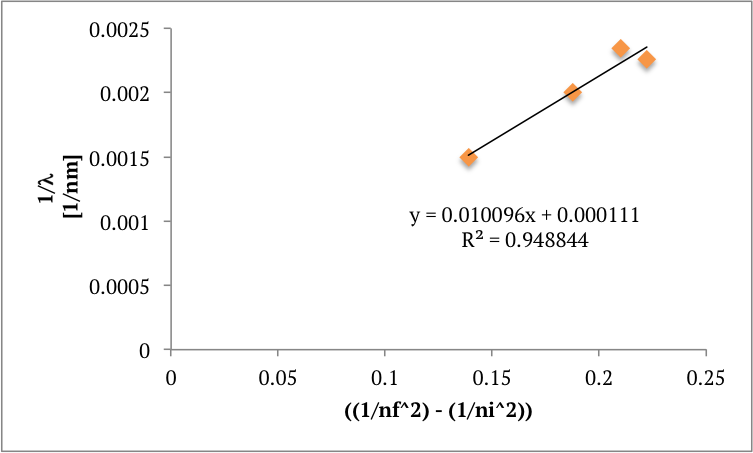
\includegraphics[scale= 0.65]{constante.png}
    \caption{Con el fin de obtener el valor de la constante de Ryderberg (con un valor teórico aproximado a $0.010973732 nm^{-1}$), se grafican los datos obtenidos para el hidrógeno y se evalúa el valor de la pendiente.}
    \label{fig:constante}
\end{figure}

La razón por la cuál se tomaron los datos únicamente del hidrógeno del cuadro \ref{tab:18} es porque presentan los menores errores. Teniendo en cuenta que el valor teórico era de $0.010973732 nm^{-1}$ y el valor experimental obtenido en la gráfica \ref{fig:constante} fue de $0.010096 nm^{-1}$, se puede decir que el valor encontrado tiene un error de $7.998\%$. Este error es muy bajo teniendo en cuenta el método de medición utilizado para obtener los datos sufre de muchas fuentes de error como son el paralaje o la incertidumbre asociada a la regla. Esto puede ser evaluado conforme a la linealidad de la gráfica \ref{fig:constante} dado que el coeficiente de correlación fue de 0.948844, con un error de $5.116\%$. Éste error demuestra que existen fuentes de error aleatorias adicionales a las sistemáticas que afectan directamente el resultado.

\begin{table}[H]
  \centering
  \caption{L de $149.2 \pm 0.1 cm$. Los datos obtenidos y asumidos como teóricos provienen de la base de datos de la NIST \cite{NIST}.}
    \begin{tabular}{|r|r|r|r|r|}
    \hline
    \multicolumn{1}{|l}{$\lambda$ NIST [nm]} & \multicolumn{1}{|l}{Inc. [nm]} & \multicolumn{1}{|l}{$\lambda$ exp. [nm]} & \multicolumn{1}{|l}{Inc. [nm]} & \multicolumn{1}{|l|}{Error ($\%$)} \\
    \hline
    \multicolumn{5}{|c|}{Mercurio} \\
    \hline
    502.2600 & 2E-04 & 385.79 & 6.3.E-04 & 23.19 \\
    546.0750 & 9E-04 & 480.29 & 6.1.E-04 & 12.05 \\
    576.9610 & 1E-04 & 517.16 & 6.1.E-04 & 10.36 \\
    \hline
    \multicolumn{5}{|c|}{Helio} \\
    \hline
    471.31457 & 2.4E-06 & 401.16 & 6.3.E-04 & 14.88 \\
    492.19313 & 3E-06 & 442.63 & 6.2.E-04 & 10.07 \\
    587.5621 & 3E-06 & 515.24 & 6.1.E-04 & 12.31 \\
    667.8151 & 3E-06 & 584.75 & 5.9.E-04 & 12.44 \\
    \hline
    \multicolumn{5}{|c|}{Hidrógeno} \\
    \hline
    410.1734 & 2E-04 & 384.76 & 6.3.E-04 & 6.20 \\
    486.135 & 3E-04 & 435.61 & 6.2.E-04 & 10.39 \\
    656.279 & 7E-04 & 585.66 & 5.9.E-04 & 10.76 \\
    \hline
    \multicolumn{5}{|c|}{Neón} \\
    \hline
    540.05616 & 1E-04 & 478.32 & 6.2.E-04 & 11.43 \\
    585.24878 & 1E-04 & 509.46 & 6.1.E-04 & 12.95 \\
    602.99968 & 1E-04 & 536.24 & 6.0.E-04 & 11.07 \\
    621.72812 & 1E-04 & 562.56 & 5.9.E-04 & 9.52 \\
    633.44276 & 1E-04 & 585.66 & 5.9.E-04 & 7.54 \\
    \hline
    \end{tabular}%
  \label{tab:149}%
\end{table}%

En comparación con el número de datos obtenidos en el cuadro \ref{tab:18}, en el cuadro \ref{tab:149} para el mercurio se esperaban nueve valores de lambda y se obtuvieron tres, para el helio se esperaban siete valores de lambda y se obtuvieron cuatro, para el hidrógeno se esperaban cuatro valores de lambda y se obtuvieron tres, y para el neón se esperaban trece valores de lambda y se obtuvieron cinco. Al comparar con los datos anteriores se puede notar que se obtuvieron muchos menos valores para cada uno de los elementos. Esto demuestra que, no sólo en términos de calidad sino en términos de calidad hay un daño significativo en la toma de datos dependiendo de la longitud. A longitudes menores hay más posibilidad de ver líneas más nítidas y, por este mismo motivo, de tener una mayor variedad de datos con los cuáles se puede estudiar el fenómeno del espectro atómico. 

Adicionalmente, dados los errores porcentuales mostrados en el cuadro \ref{tab:18} y en el cuadro \ref{tab:149}, se puede deducir entonces que los valores obtenidos son más precisos cuando se utilizan las longitudes son menores. Cuando esto sucede, se disminuye el paralaje y se obtienen mediciones con menores errores aleatorios que parece afectar drásticamente la obtención de datos. El dato con mayor error en el cuadro \ref{tab:18} fue de $10\%$ mientras que en el cuadro \ref{tab:149} fue de $25\%$, claramente distanciados. \\

Por otro lado, en la segunda parte del experimento, se midieron los espectros de emisión de 3 LEDs: azul, verde y rojo a $V=5V$ y, para cada uno de ellos, se determinó la mínima y la máxima longitud de onda ($\lambda_{min}$ y $\lambda_{max}$, respectivamente) en la que emitían; así como la longitud de onda, $\lambda_{int}$, en la que se daba la mayor intensidad de emisión, al hacer pasar la luz por una rejilla de difracción. \\
Mediante un proceso similar al de la primera parte del experimento, se calcularon, entonces, dichas longitudes de onda, usando la ecuación \eqref{(2)}, con $m=1$, como se presenta en el cuadro a continuación.

\begin{table}[H]
\centering
  \caption{Longitud de onda mínima, máxima y de mayor intensidad ($\lambda_{min-exp}$, $\lambda_{max-exp}$ y $\lambda_{int}$ respectivamente) para LEDs verde (G), azul (B) y amarillo (Y). En la tabla se presentan, también, los valores teóricos para $\lambda_{min-teo}$ y $\lambda_{max-teo}$ \cite{LEDs_lambda}.}
  \begin{adjustbox}{width=8.5cm}
\begin{tabular}{|c|c|c|c|c|c|}
\hline
$ $        & $\lambda_{min-teo}[nm]$ & $\lambda_{min-exp}[nm \pm 10]$ & $\lambda_{int}[nm \pm 10]$ & $\lambda_{max-exp}[nm \pm 10]$ & $\lambda_{max-teo}[nm]$ \\ \hline
G    & 500            & 502,31     & 527,93     & 582,43     & 570            \\ \hline
B     & 395      & 414,56     & 467,33     & 503,75     & 500            \\ \hline
Y & 570            & 574,99     & 579,46     & 598,50     & 590            \\ \hline
\end{tabular}
\label{tableds}
 \end{adjustbox}
\end{table}

Como se puede contemplar en la tabla, los valores obtenidos para el rango en el cual cada LED tiene su espectro de emisión es bastante exacto respecto al valor teórico, mostrado en \cite{LEDs_lambda}. No obstante, puede observarse que, para los tres LEDs, el valor mínimo de la longitud de onda experimental, $\lambda_{min-exp}$, está un poco desfasado respecto a  $\lambda_{min-teo}$. Esto se debe a varios errores asociados a la práctica; en los que, al parecer, si visualizó que el espectro de emisión era más corto de lo que realmente es. 
\\
En el caso del LED verde, por ejemplo, para $\lambda_{min}$, se tiene un error experimental de apenas el $\epsilon = 0,462 \%$; y, para $\lambda_{max}$, uno del $\epsilon = 2,134 \%$. Claramente, los errores asociados son bastante bajos, lo cual indica que el experimento fue bastante exacto. Asimismo, vale la pena aclarar que, posiblemente, el error experimental esté dado por errores asociados a la medición; en los que, por ejemplo, en el caso de $\lambda_{max}$, se alcanzaban a confundir como verdes los primeros tonos de amarillo del espectro, tomando medidas inadecuadas con errores aleatorios asociados. No obstante, es necesario establecer que $\lambda_{int}$ tiene un valor adecuado; pues tiene sentido pensar que la mayor intensidad lumínica a la que emite el LED no sólo está entre $\lambda_{min}$ y $\lambda_{max}$; sino que, también, toma un valor intermedio entre ambos extremos. \\
Para el LED azul, se tuvo un error experimental para  $\lambda_{min}$ de apenas el $\epsilon = 4,95 \%$; y, para $\lambda_{max}$, uno del $\epsilon = 0,75 \%$. Claramente, los errores asociados son bastante bajos, lo cual indica que el experimento fue bastante exacto. Asimismo, vale la pena aclarar que, posiblemente, el error experimental esté dado por errores asociados a la medición; en los que, por ejemplo, en el caso de $\lambda_{min}$, se alcanzaban a confundir como azules los últimos tonos de morado del espectro (los más cercanos al espectro ultravioleta - UV), tomando medidas inadecuadas con errores aleatorios asociados. No obstante, es necesario establecer que $\lambda_{int}$ tiene un valor adecuado; pues tiene sentido pensar que la mayor intensidad lumínica a la que emite el LED no sólo está entre $\lambda_{min}$ y $\lambda_{max}$; sino que, también, toma un valor intermedio entre ambos extremos. \\
Por último, para el LED amarillo, se tuvo un error experimental para  $\lambda_{min}$ de apenas el $\epsilon = 0,172 \%$; y, para $\lambda_{max}$, uno del $\epsilon = 1,44 \%$. Claramente, los errores asociados son bastante bajos, lo cual indica que el experimento fue bastante exacto. Asimismo, vale la pena aclarar que, posiblemente, el error experimental esté dado por errores asociados a la medición; en los que, por ejemplo, en el caso de $\lambda_{max}$, se alcanzaban a confundir como amarillos los primeros tonos de rojo del espectro (los más cercanos al espectro infrarrojo - IR), tomando medidas inadecuadas con errores aleatorios asociados. No obstante, es necesario establecer que $\lambda_{int}$ tiene un valor adecuado; pues tiene sentido pensar que la mayor intensidad lumínica a la que emite el LED no sólo está entre $\lambda_{min}$ y $\lambda_{max}$; sino que, también, toma un valor intermedio entre ambos extremos. 

\section{\label{sec:conclusiones} Conclusiones}

En conclusión, todos los objetivos fueron cumplidos con satisfacción. Primero, se midieron las longitudes de onda emitidas por un átomo de hidrógeno con dos longitudes distintas, como se muestran en los cuadros \ref{tab:18} y \ref{tab:149}. Utilizando una distancia más corta se lograron encontrar los cuatro valores buscados asociados al espectro de emisión de éste elemento. Se comprobó, adicionalmente que tener una mayor longitud aumenta el error aleatorio y el paralaje, ya que disminuye el número de líneas nítidas visibles y afecta la precisión de los datos obtenidos. Utilizando los datos más precisos se lograron conseguir datos con errores menores al $10\%$, despreciables para el desarrollo del experimento. Gracias a esto, se comprobó que se ajustan los datos a la fórmula de Balmer gracias a la regresión lineal dibujada en la gráfica \ref{fig:constante}. El coeficiente de correlación es aceptable, con un valor total de 0.9488. 

Segundo, se utilizó la ecuación \eqref{BalmerMejorada} para definir los parámetros de la gráfica obtenida. Según dicha ecuación, la pendiente de la gráfica \ref{fig:constante} debería ser igual a la constante de Ryderberg, que tiene un valor aproximado de $0.010973732 nm^{-1}$. En nuestra gráfica \ref{fig:constante} se obtuvo una pendiente de $0.010096 nm^{-1}$ con un error de $7.998\%$. Este error podría considerarse bajo teniendo en cuenta que nuestros datos tuvieron un error del $5.116\%$ conforme al análisis del coeficiente de correlación. Teniendo en cuenta diversas fuentes de error como el paralaje y la incertidumbre asociada al instrumento de medida, se dice entonces que el error experimental es aceptable y que se midió con éxito la constante buscada.

Tercero, se midieron algunas líneas espectrales de otros elementos, a saber, del mercurio, el helio, el neón y el argón. Se logró evidenciar cómo, dependiendo de la cercanía de las longitudes de onda características de cada elemento, se logran mostrar más o menos líneas espectrales. Adicionalmente, se muestra cómo el rango en el que cierto elemento emite las longitudes de onda depende meramente de la composición del elemento y cómo hay un espectro distinto para cada elemento. Los datos encontrados más precisos se encuentran en el cuadro \ref{tab:18}. 

Por último, se midieron las longitudes de onda emitidas por tres LEDs: uno verde, uno amarillo y uno azul. Para cada uno de ellos, se determinó su longitud de onda $\lambda_{int}$ en la que se emitía la mayor luminosidad (en el rango del espectro emitido por el LED, entre $\lambda_{min}$ a $\lambda_{max}$), a una distancia, \textit{L}, determinada. Estas longitudes de onda obtenidas se compararon con los valores aceptados por la teoría (ver \cite{LEDs_lambda}, como se ve detalladamente en el cuadro \ref{tableds}. Aunque se hayan obtenido valores bastante cercanos a los aceptados, los errores aleatorios asociados al experimento (sobre todo, a la visión del espectro generado por la rejilla de difracción) hicieron que, en los tres casos, se alcanzara a obtener un rango de longitudes de onda un poco mayores a los teóricos. Esto hizo, entonces, que algunas longitudes de onda de los rangos obtenidos, correspondieran al rango de luz visible inmediatamente siguiente para el verde y el amarillo (correspondiente al amarillo y rojo, respectivamente); y, en el caso del azul, al inmediatamente anterior (correspondiente a los morados y violetas). No obstante, a pesar de lo anterior, el experimento fue bastante preciso y exacto y cumplió con los objetivos planteados en este laboratorio, correspondientes a la medición de la longitud de onda emitida por LEDs.



\bibliography{biblio}

\end{document}